\documentclass{article}
\usepackage[a4paper,left=15mm,right=15mm,top=5mm,bottom=15mm]{geometry}
\usepackage{amssymb,amsthm,latexsym,amsfonts, amsmath, bm}
\usepackage[lined,ruled]{algorithm2e}
\usepackage{extarrows}
\usepackage{enumerate}
\usepackage{tikz}
\usepackage{underoverlap}
\usepackage{xcolor}
\usepackage{graphicx}
\usepackage{float}
\newtheorem{lemma}{Lemma}
\newtheorem{theorem}{Theorem}
\title{Exercises for Algorithmic Bioinformatics II\\
Assignment 1}
\author{Xiheng He}
\date{November 2021}
\linespread{1.5}
\begin{document}
\flushright{Wintersemester 2021/22}
\flushleft{Xiheng He}
\flushleft{Lisanne Friedrich}
{\let\newpage\relax\maketitle}
\begin{flushleft}
\textbf{Exercise 2 (Fibonacci, 15P):}
\begin{enumerate}[(a)]
    \item  Implement the different algorithmic versions.
    \newline All Implementations in Fibonacci.jar of moodle website.
    \item  Fibonacci numbers grow quite fast and become big. How many Fibonacci numbers can you
    compute with 32bit, 64bit and 128bit integers?
    \newline
    Apply Binet's formula:
    \begin{equation}
        F(n) = \frac{\varphi^n - \psi ^n}{\sqrt{5}}
    \end{equation}
    \begin{equation}
        \varphi = \frac{1 + \sqrt{5}}{2}
    \end{equation}
    \begin{equation}
        \psi = \frac{1 - \sqrt{5}}{2}
    \end{equation}
    \begin{itemize}
        \item 32 bit integer: $2^{32} - 1 = 4294967295$ 
        \newline
        \begin{align*}
        F(n) \leq 2 ^ {bit} \Longrightarrow
        \varphi ^ n \leq \sqrt{5} \cdot 2 ^ {bit} \quad (\psi ^ n < 1) \\ 
        \Longrightarrow n \cdot \log \varphi \leq {bit} \cdot \log 2 + \frac{1}{2} \cdot \sqrt{5} \\
        \Longrightarrow n \leq {bit} \cdot \frac{\log 2}{\log \varphi} + \frac{\log 5}{2 \log \varphi} \\
        bit := 31 \Longrightarrow n \leq 32 \cdot 1.44 + 1.67 \approx 46
        \end{align*}
        maximal $F(46)$ can be computed with 32 bit integer.
        \item 64 bit integer: $2^{64} - 1 = 18,446,744,073,709,551,615$
        \begin{align*}
            bit := 63 \Longrightarrow n \leq 63 \cdot 1.44 + 1.67 \approx 92
        \end{align*}
        maximal $F(92)$ can be computed with 64 bit integer.
        \item 128 bit integer $2^{128} - 1 = 	340,282,366,920,938,463,463,374,607,431,768,211,455$
        \begin{align*}
            bit := 127 \Longrightarrow n \leq 127 \cdot 1.44 + 1.67 \approx 184
        \end{align*}
        maximal $F(184)$ can be computed with 128 bit integer.
    \end{itemize}
    \item Analyse your implementations. How many function calls are needed? How many additions,
    multiplications? How does that correlate with the actual runtime of the implementation?
    How is the growth of the Fibonacci numbers? Give estimations, proofs and visualizations as
    evidence for your findings!  
    \begin{itemize}
        \item iterative version: for a 3 till $n$ loop addition = 1
        \begin{align*}
            T(n) = (n - 3 + 1) \cdot 1 = O(n)
        \end{align*}
        \item recursive version: for each $T(k)$ addition = 1
        \begin{align*}
            T(n) &= T(n - 1) + T(n - 2) \\
            &= 2(T-2 + 1) \\
            &= 2(2(n - 2) + 1) + 1 = 4T(n - 2) + 3 \\
            &= 2^k \cdot T(n - k) + 2^k - 1 \\
            &= 2^n \cdot T(0) + 2^n - 1 \\
            &= 2^n + 2^n - 1 = O(2^n)
        \end{align*}
        \item logarithmic version: for each $T(n), T(\frac{n}{2})$ must be calculated, addition = 1, multiplication = 2 
        \begin{align*}
            T(n) &= T(\frac{n}{2}) + 4 \\
            \Longrightarrow k &:= \log n \Longrightarrow T(2^k) = T(2^ {k - 1}) + 4 \\ 
            \Longrightarrow T(n) &= T(0) + 4k \Longrightarrow T(n) = O(\log n)
        \end{align*}
    \end{itemize}
    \begin{figure}[H]
        \centering
        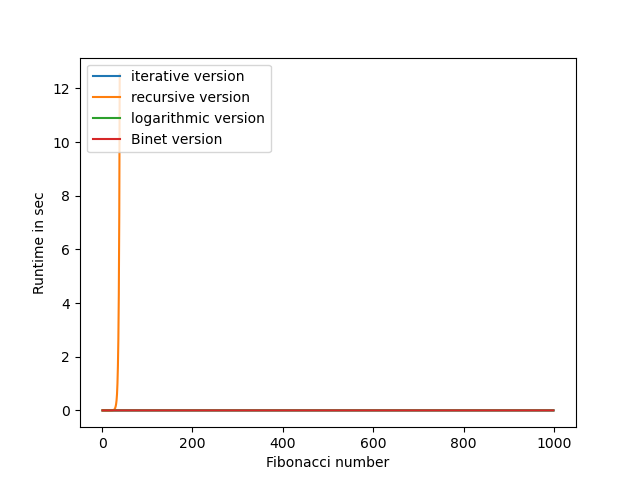
\includegraphics{benchmarking.png}
        \caption{benchmark of all approaches}
    \end{figure}
    \begin{figure}
        \centering
        \begin{minipage}{0.48\textwidth}
        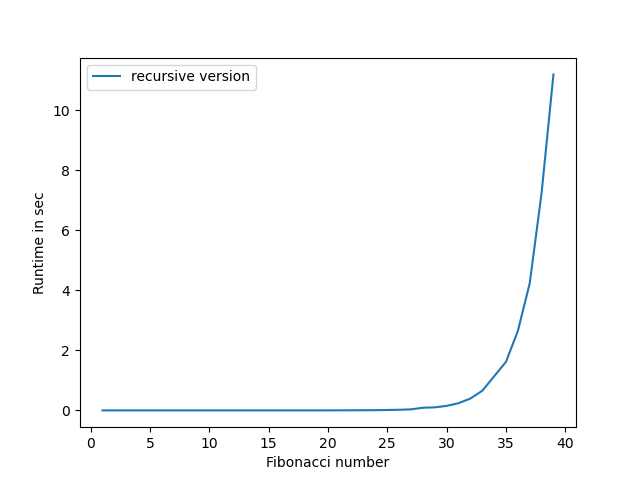
\includegraphics[width=8.5cm]{recursive_only.png}
        \caption{recursive version}
        \end{minipage}
        \centering
        \begin{minipage}{0.48\textwidth}
        \centering
        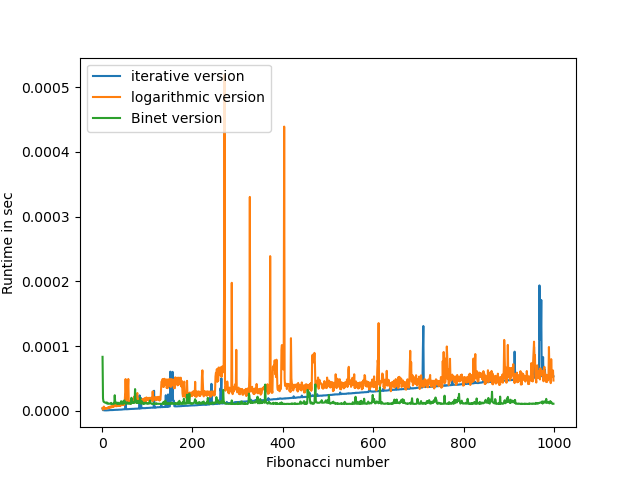
\includegraphics[width=8.5cm]{no_recursive.png}
        \caption{benchmark without recursive version}
        \end{minipage}
    \end{figure}
    \item  There is an “explicit” formula (Binet, 1843) for computing Fibonacci numbers. Prove this
    formula (by induction) and implement it. Then compare this version with your other implementations. 
    How efficient is your implementation of this formula?  
    \newline
    Prove Binet formula by by induction:
    \begin{equation}
        F(n) = \frac{\varphi^n - \psi ^n}{\sqrt{5}}
    \end{equation}
    \begin{equation}
        \varphi = \frac{1 + \sqrt{5}}{2}
    \end{equation}
    \begin{equation}
        \psi = \frac{1 - \sqrt{5}}{2}
    \end{equation}
    \begin{itemize}
        \item Base case: 
        \begin{align*}
            n &= 0: f(0) = 0 \\ 
            n &= 1: f(1) = \frac{\frac{1 + \sqrt{5}}{2} - \frac{1 - \sqrt{5}}{2}}{\sqrt{5}} = 1
        \end{align*}
        \item Inductive hypothesis:
        \begin{align*}
            \forall n \geq 0, F(n) = \frac{\varphi^n - \psi ^n}{\sqrt{5}}
        \end{align*}
        \item Inductive step: $n \longrightarrow n + 1$
        \begin{align*}
            F(n + 1) &= F(n) + F(n - 1) \\
            &= \frac{\varphi^{n-1} - \psi^{n - 1}}{\sqrt{5}} + \frac{\varphi^n - \phi^n}{\sqrt{5}} \\
            \because \varphi ^ 2 &= \varphi + 1 \Longrightarrow \varphi ^ {n + 1} = \varphi ^ n + \varphi ^ {n - 1} \\
            \therefore F(n) + F(n - 1) &= \frac{\varphi^{n + 1} - \phi^{n + 1}}{\sqrt{5}} = F(n + 1) \qed
        \end{align*}
        \newline
        Binet's formula runs in $O(n)$. 
    \begin{figure}[H]
        \centering
        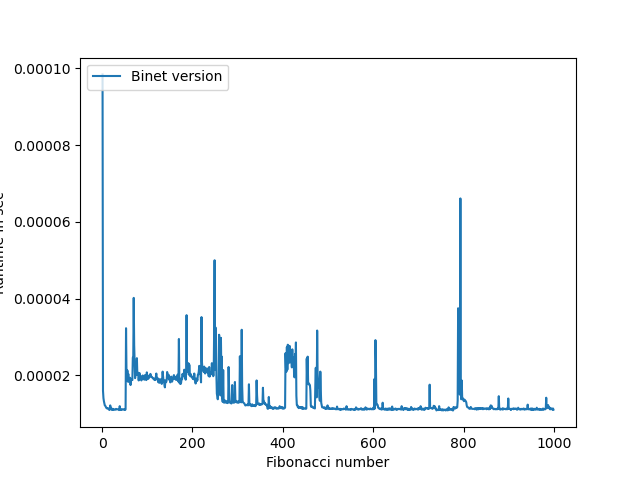
\includegraphics{binet.png}
        \caption{Binet's formula}
    \end{figure}
    As we can see, the performance of Binet's approach is not quite stable.
    \end{itemize}
\end{enumerate}    
\end{flushleft}
\end{document}